\documentclass{report}
\usepackage{amsmath}
\usepackage{geometry}
\usepackage{graphicx}
\begin{document} 

\begin{flushleft}

\begin{Large}

\textbf{Name - Ankush Vijay Israney} \\
\textbf{Student ID - 14057308} \\
\textbf{CS 613 - Assignment 4 report} \\ 

\end{Large} 

\break

\section{\underline{part1}}
\underline { \textbf{BINARY ARTIFICIAL NUERAL NETWORKS}}  \linebreak[2]

\textbf{Test Error = 0.0875} 

\begin{figure}[tph!]
\centering
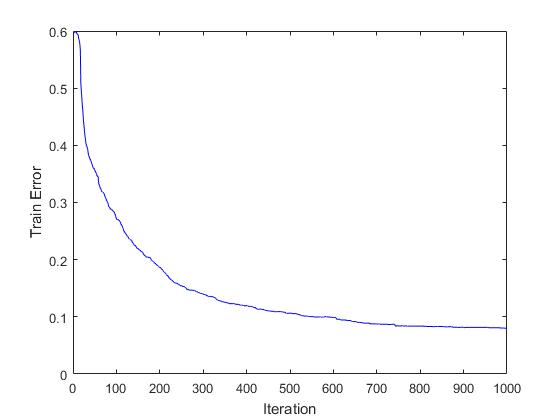
\includegraphics{part1.jpg}
\end{figure}

\break

\section{\underline{part2}}
\underline { \textbf{THE PRECISION-RECALL TRADEOFF}}  

\begin{figure}[ht!]
\centering
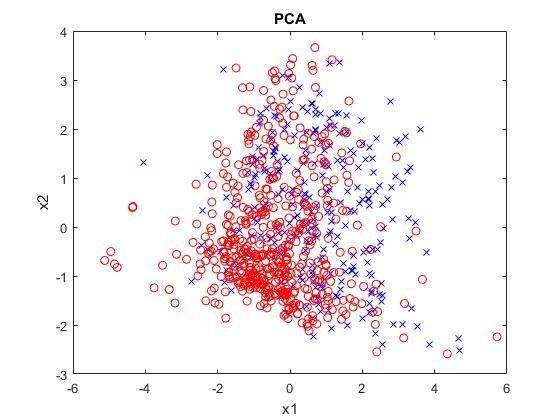
\includegraphics{part2.jpg}
\end{figure} 

\break

\section{\underline{part3}}
\underline { \textbf{MULTI-CLASS ARTIFICIAL NUERAL NETWORKS}}  \linebreak[2]

\textbf{Test Error = 0.1103} 

\begin{figure}[tph!]
\centering
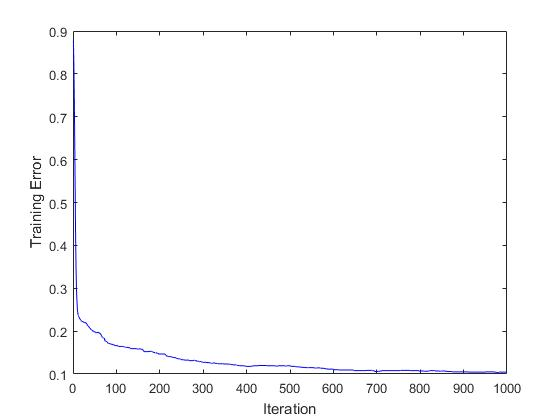
\includegraphics{part3.jpg}
\end{figure}



\end{flushleft} 

\end{document}